\documentclass{beamer}

%\usepackage[utf8x]{inputenc}
\usepackage{textcomp}
%\usepackage{graphicx}
%\usepackage{subcaption}
%\usepackage{floatrow}
\usepackage{subfig}
\usepackage{array}

\definecolor{OSUdkbrn}{RGB}{104,80,64}
\definecolor{OSUmedbrn}{RGB}{176,96,16}
\definecolor{OSUltbrn}{RGB}{224,195,152}
% from: http://oregonstate.edu/brand/color-palette


\usepackage[backend=biber,citestyle=authoryear,bibstyle=authoryear,maxbibnames=10]{biblatex}
\addbibresource{../report/VCPbibliography.bib}

\mode<presentation>
{
	\usetheme{CambridgeUS}
	\setbeamercovered{transparent}
	\setbeamertemplate{footline}[page number]{}
	\setbeamertemplate{navigation symbols}{} % remove navigation symbols
	\setbeamercolor{palette tertiary}{fg=white, bg=OSUdkbrn}
	\setbeamercolor{title}{fg=OSUdkbrn}
	\setbeamercolor{frametitle}{fg=OSUdkbrn}
	\setbeamertemplate{itemize items}[square]
	\setbeamercolor*{item}{fg=OSUdkbrn}
%	
%	\setbeameroption{show only notes} % ----------------------- NOTES TOGGLE ---------------------
%
}

\title{Variable Circular Plots: Station Placement and the Independence Assumption}
\subtitle{Master's Research Project}
\author{Matt Edwards}
\date{June 11, 2014}

\begin{document}
\begin{frame}
	\titlepage
\end{frame}

%\begin{frame}
%	\frametitle{Outline}
%	\tableofcontents
%\end{frame}

% -------------------------------- INTRODUCTION --------------------------------------------------
\section{Introduction}

\begin{frame}{Distance Sampling}
Distance sampling is a method of population density estimation that considers the probably of observing the object of interest at the distance at which it was seen.

	\begin{itemize}
	\item Used often in Ecological Sciences
	\item[]
	\item Began with roadside surveys in early 1900s
	\item[]
	\item Theory developed through mid-1900s
	
	\end{itemize}
\end{frame}

\begin{frame}{Distance Sampling: History}
A selection of relevant papers:
	\begin{itemize}
	\item Emlen---1971
	\item Ramsey, Scott---1979, 1980 Papers
	\item Burnham, Anderson, and Jeffrey L. Laake---1980 Monograph
	\item Buckland et. al. 1993, 2001---text
	\item Continued Development into 2000s
	\begin{itemize}
	\item Combined with Mark-Recapture Methods
	\item Extended for use with underwater acoustics for estimates of krill populations 
	\item Combined with camera traps to estimate populations
	\end{itemize}
	\end{itemize}
\end{frame}

\begin{frame}{Line vs Point Transects}
	\begin{itemize}
	\item Line transects are walked
	\begin{itemize}
		\item Distances perpendicular to transect are recorded, as projected on ground
	\end{itemize}
	\item[]
	\item Point transects: observer(s) stand at station, observe everything within 360\textdegree 
		\begin{itemize}
		\item Alternately: Variable Circular Plots (VCP)
		\item Allow ``cooling'' period
		\item Safer for observer
		\item Straight line distance from Observer is recorded, as projected on ground
		\end{itemize}
	\item[]		
	\item Both: Observations can be from visual sightings, auditory clues, or a combination
	\end{itemize}
\end{frame}

\begin{frame}{Transect Examples}

	\begin{columns}
		\begin{column}{0.48\textwidth}
		\centering
		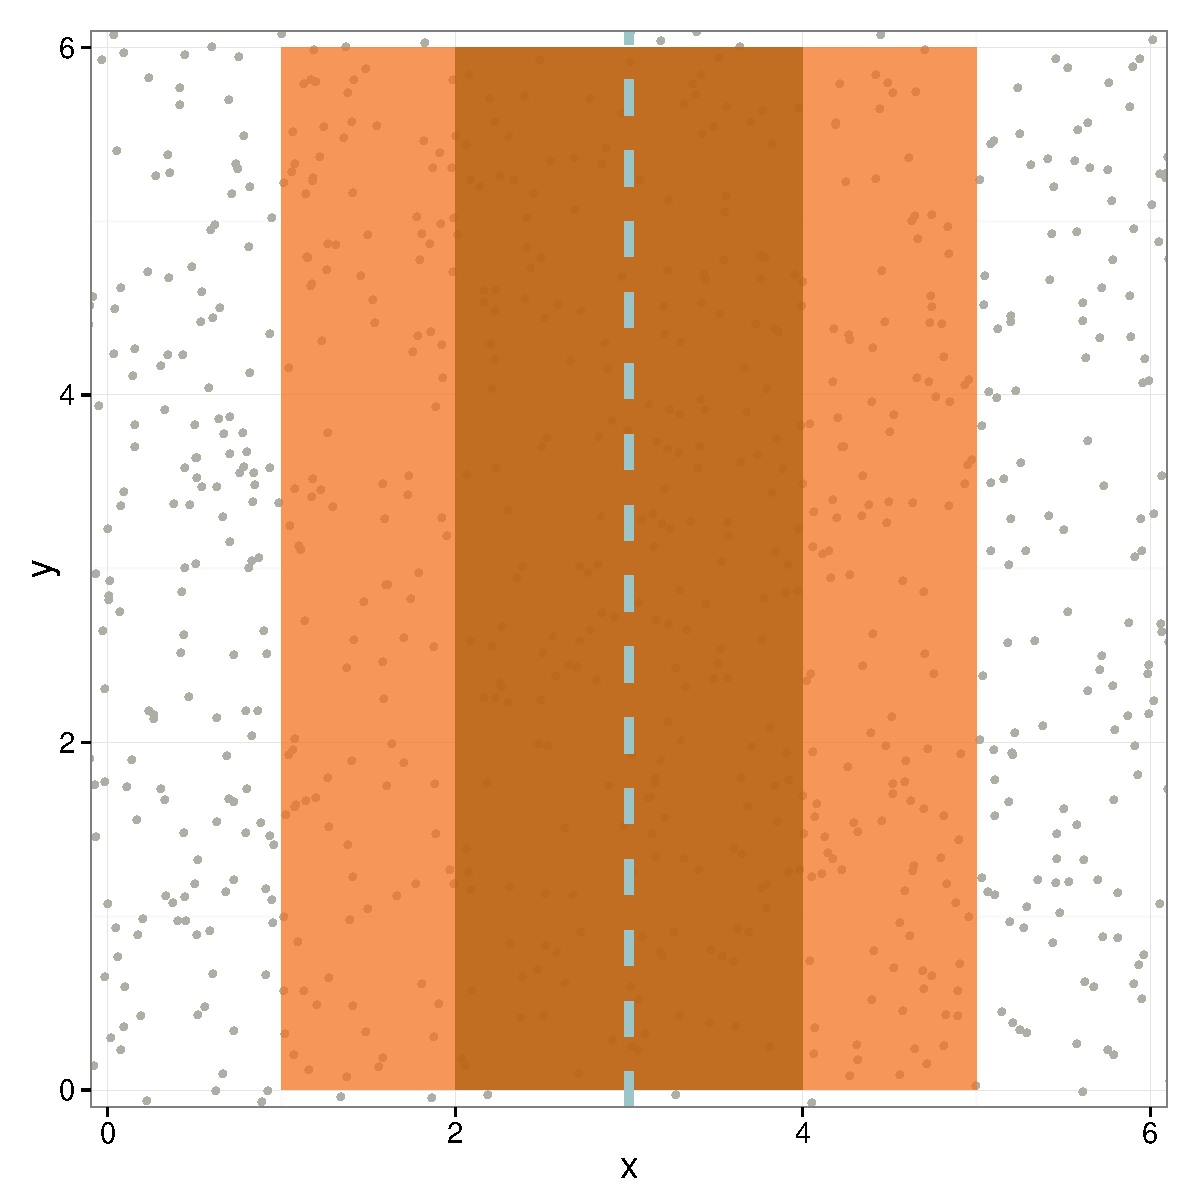
\includegraphics[width=\textwidth]{../images/slides-LTr.pdf}\\
		Line Transect
		\end{column}
		\begin{column}{0.48\textwidth}
		\centering
		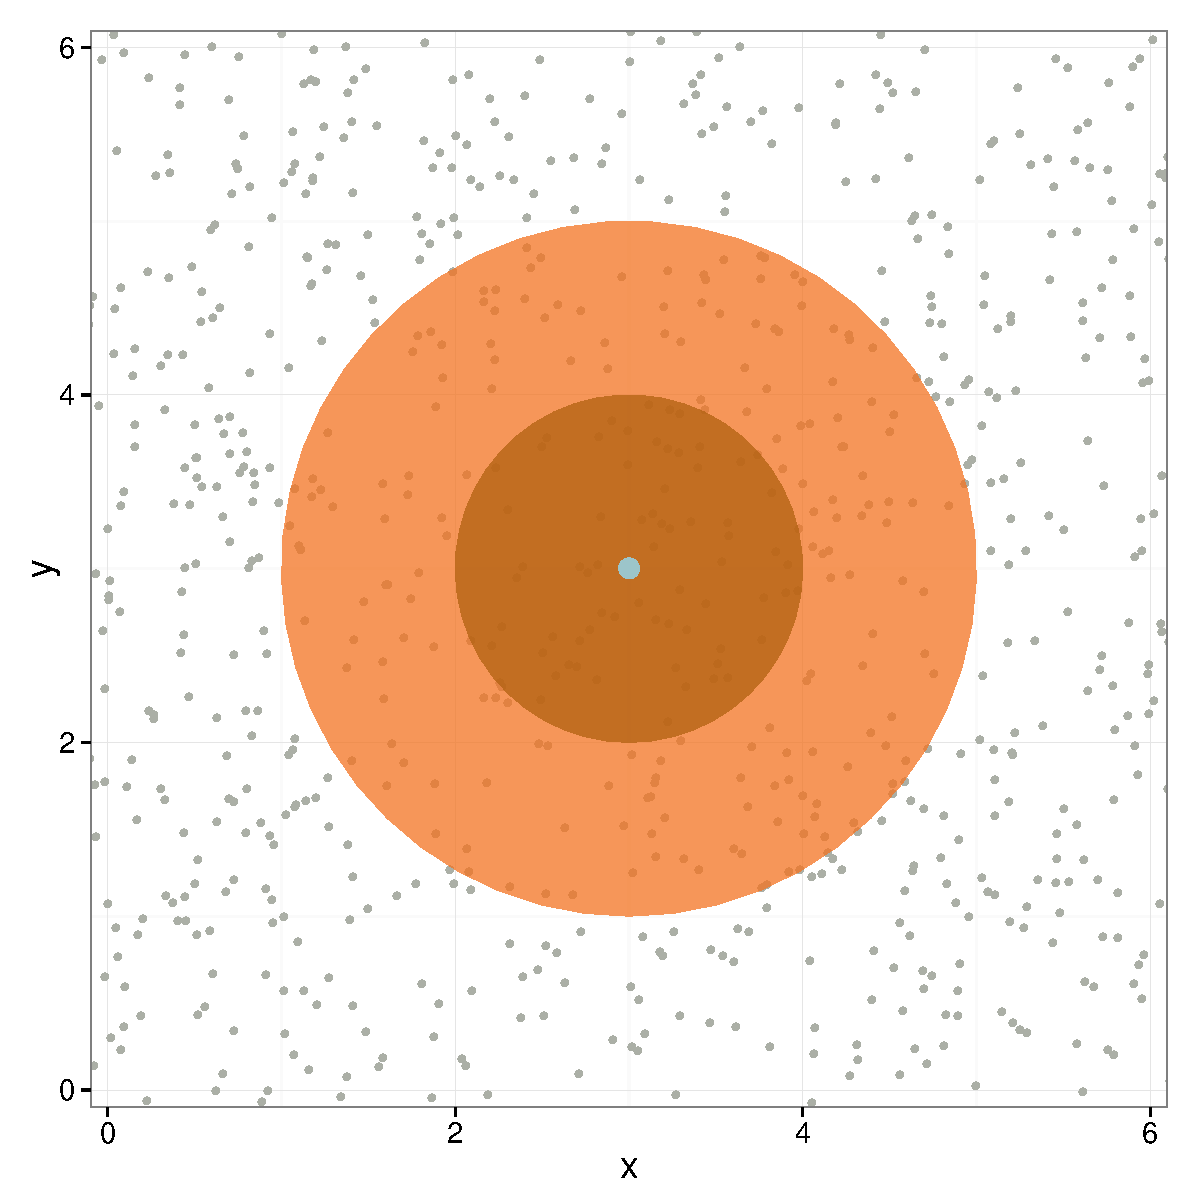
\includegraphics[width=\textwidth]{../images/slides-VCPr.pdf}\\
		VCP/Point Transect
		\end{column}
	\end{columns}

\end{frame}

\begin{frame}{Detection Curve: $g(r)$}
The probability of detecting an object, give it is at distance $r$.
	\begin{figure}
		\centering
		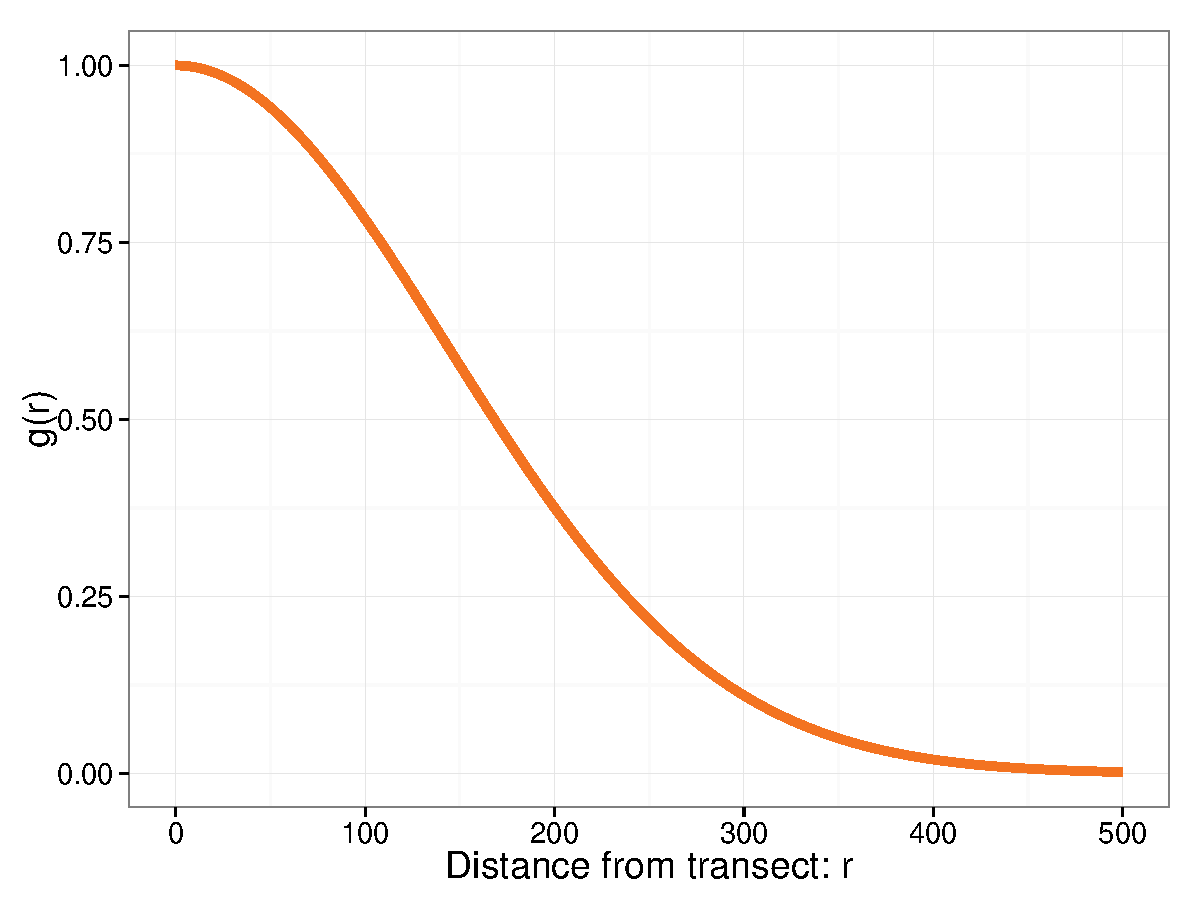
\includegraphics[width=\textwidth,height=0.80\textheight,keepaspectratio=true]{../images/detectionCurve.pdf}
	\end{figure}
	\note{
		\begin{itemize}
		\item Perfect Detectability Near to Observer, dropping off. The ``shoulder''
		\item $g(r)$ = probability of detecting an object, given it is at distance $r$
		\item scaled so $g(0) = 1$
		\end{itemize}
	}
\end{frame}

\begin{frame}{Density Estimation}
	\begin{center}
	$\hat{D}=\dfrac{n}{\mbox{Area}*P(\mbox{observing object}|\mbox{distance }r)}$\\
	\vspace{0.5cm}
	$\hat{D}=\dfrac{n}{\mbox{Area}*g(r)}$
	\end{center}
	
	\begin{itemize}
	\item $\hat{D}$: Estimated Population Density
	\item $n$: number of objects observed
	\item $Area$: The area surveyed
	\item $g(r)$: $P(\mbox{observing object}|\mbox{distance }r)$
	\end{itemize}

	\note{
		\begin{itemize}
		\item Much of the difficulty in distance sampling comes from estimating g(r)
		\item For this presentation, the kernel method, a non-parametric method, was used.
		\item in very broad terms, it looks at the average count per VCP and estimates area and probability by averaging over the observed observation distances inside a normal kernel. 
		\end{itemize}
	}
\end{frame}

% -------------------------------- Micronesian Study --------------------------------------------------
\section{Micronesian Study}

\begin{frame}{Micronesian Forest Bird Survey: 1982}
\begin{itemize}
\item Engbring, Ramsey \& Wildman (1986)
\item[]
\item Used VCP to survey several bird species in the Micronesian islands
\item[]
\item Each of 5 Islands divided into regions
\item[]
\item Transect randomly placed within region (angle \& starting position selected randomly)
\item[]
\item Stations placed every 150 m along transect
\item[]
\item Additional transects placed 2 km parallel
\end{itemize}

	\note{
	\begin{itemize}
	\item Observers would wait 2 minutes after arrival, then spend 8 minutes observing all they could
	\item Distance and species were noted, as well as foliage and other variables.
	\end{itemize}
	}
\end{frame}

\begin{frame}{Micronesia}
	\begin{figure}
		\centering
		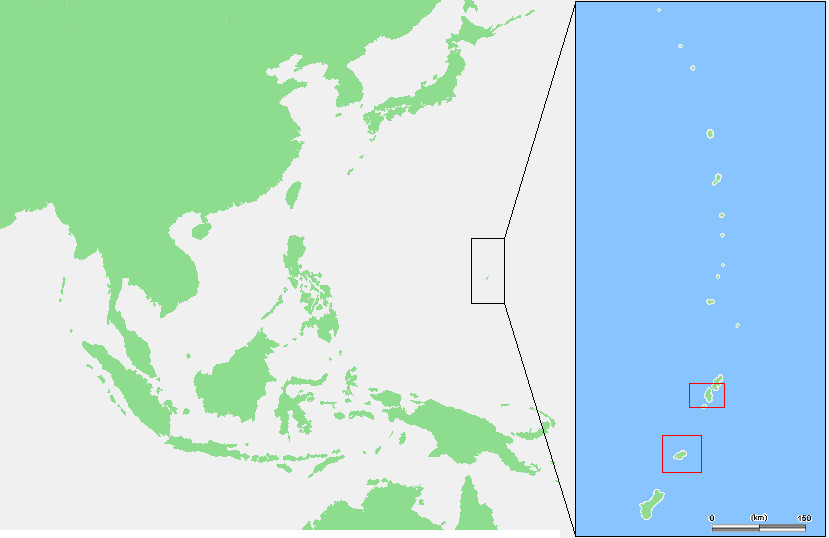
\includegraphics[height=.80\textheight]{../images/islands.jpg}
	\end{figure}
	\tiny
	\begin{center}\color{OSUdkbrn}
	Mariana Islands, modified from work by M. Minderhoud, (public domain) via  Wikimedia Commons
	\end{center}

\end{frame}

\begin{frame}{Collared Kingfisher Observation Data}
Aggregated empirical observation distances from 1982 study.
\begin{figure}
	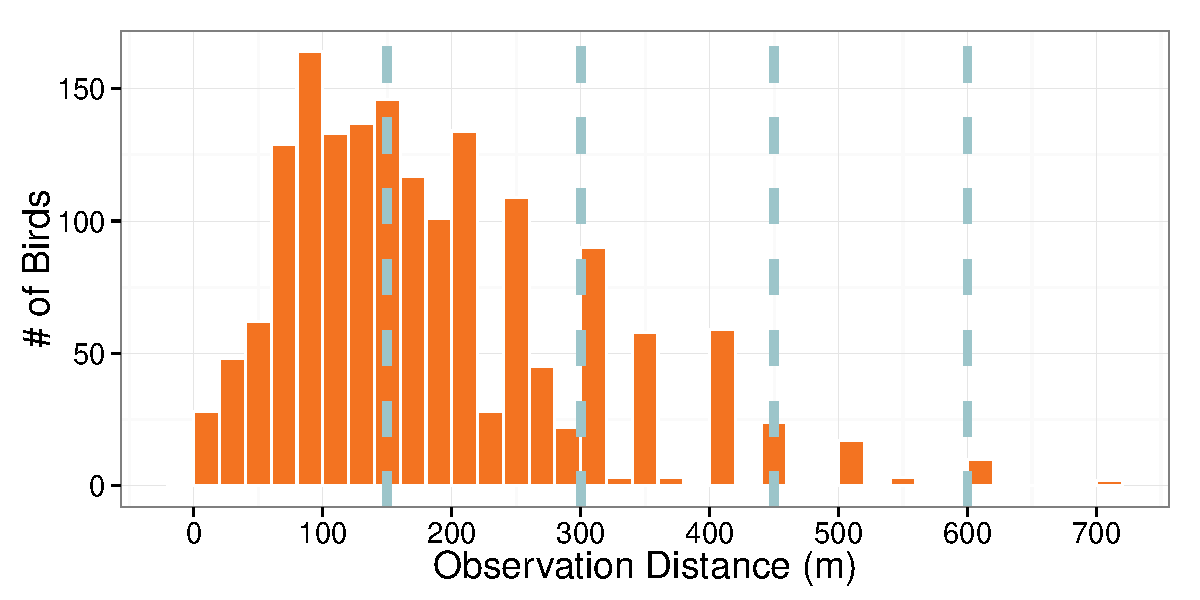
\includegraphics[width=\textwidth]{../images/histogram_dist_20m.pdf}
	\label{fig:82dist}
\end{figure}

	\note{
		\begin{itemize}
		\item Aggregated over two islands, Rota \& Tinan
		\item Aggregated over all observers, 4
		\item Primarily auditory cues, some visual, and some heard-then-seen
		\item Data tell us 3 main things
		\begin{itemize}
			\item Very low bird counts immediately around the station. Some evidence of movement.
			\item Evidence of heaping, the further away from station. More prominent with smaller bins.
			\item Stations places 150 Meters Apart.
		\end{itemize}
		\end{itemize}
	}
\end{frame}

\begin{frame}{Research Question}
\Large
{\bfseries Do overlapping observation areas violate any underlying independence assumptions?}\\
\vspace{1cm}
{\bfseries Will it make a difference in our final population density estimates if a bird is observed from more than one station?}
\end{frame}

\begin{frame}{VCP Indepencence}
	VCP Analysis assumes sightings of animals are independent events.
	\begin{itemize}
	\item[]
	\item \textcite{ramsey1979,buckland1987,thompson2012} discuss assumption that VCPs are randomly placed.
	\begin{itemize}
	\item Implicit, but not explicit, possibility of overlap
	\end{itemize}
	\item[]
	\item \textcite{reynolds1980} state the possibility of observing the same bird from more than one station should be avoided.
	\item[]
	\item \textcite{buckland2001} states ``Transects are normally spaced at a sufficient distance to avoid detecting an object from two neighboring transects, although this is not usually critical unless sampling a line changes the animal distribution at neighboring, as yet un-sampled lines.''
	\end{itemize}
	
		\note{
			\begin{itemize}
			\item Some Selected Quotes
			\item Literature is divided
			\item Transect layouts, similar to Micronesian study, are common
			\item We as scientists need to understand how this might bias our results.
			\item if layout is going to bias our results, then we need to be aware of that, so adjustments can be made to survey design or analysis. 
			\end{itemize}
		}
\end{frame}

% -------------------------------- SIMULATION --------------------------------------------------
\section{Simulation}

\begin{frame}{Simulation Set Up}
	Modeled after Palie Region on Rota:
	
	\begin{itemize}
	\item[]
	\item 20 birds per km$^2$
	\item[]
	\item 9.41 km$^2$ Study Area
	\item[]
	\item Two transects, 16 \& 17 stations each
	\item[]
	\item Truncation distance, $w$, taken to be 500 m
	\end{itemize}
	\note{
	\begin{itemize}
	\item 	Mainly because a density of 20/km$^2$ was a nice round number.
	\item There is only 0.9 \% of data beyond 500 m
	\item let me deal with nicer numbers, while still adhering to the spirit of the original data.
	\end{itemize}

	}
\end{frame}

\begin{frame}{Transect Layouts}
Examples of two random Transect layouts.\\
1 unit on graph = 1 km
	\begin{columns}
		\begin{column}{0.48\textwidth}
			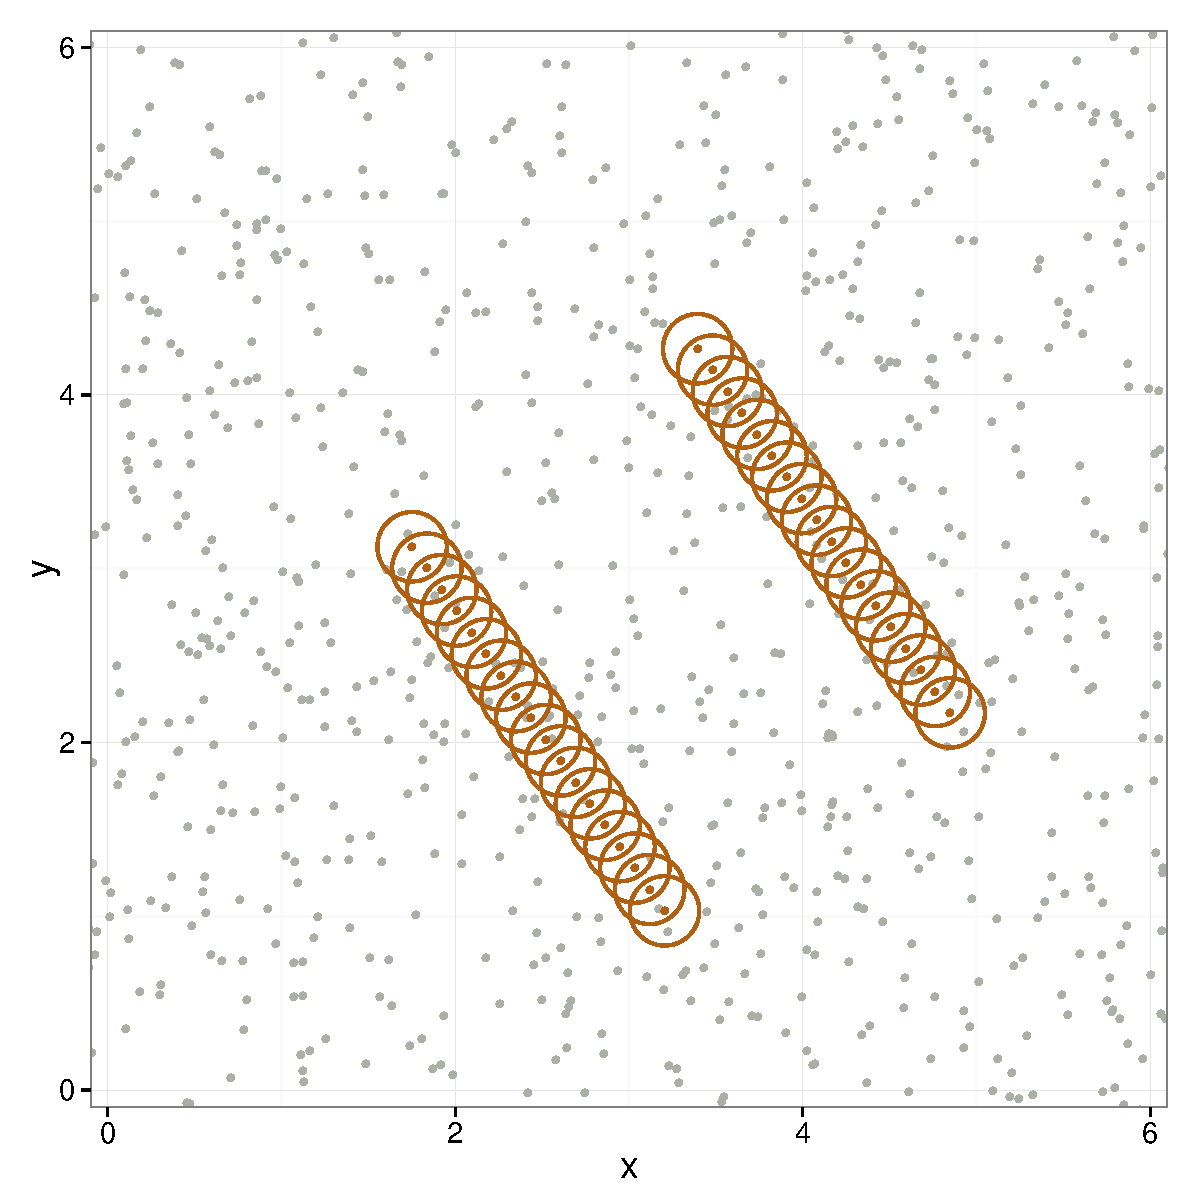
\includegraphics[width=\textwidth]{../images/slides-layoutT2.pdf}
		\end{column}
		\begin{column}{0.48\textwidth}
			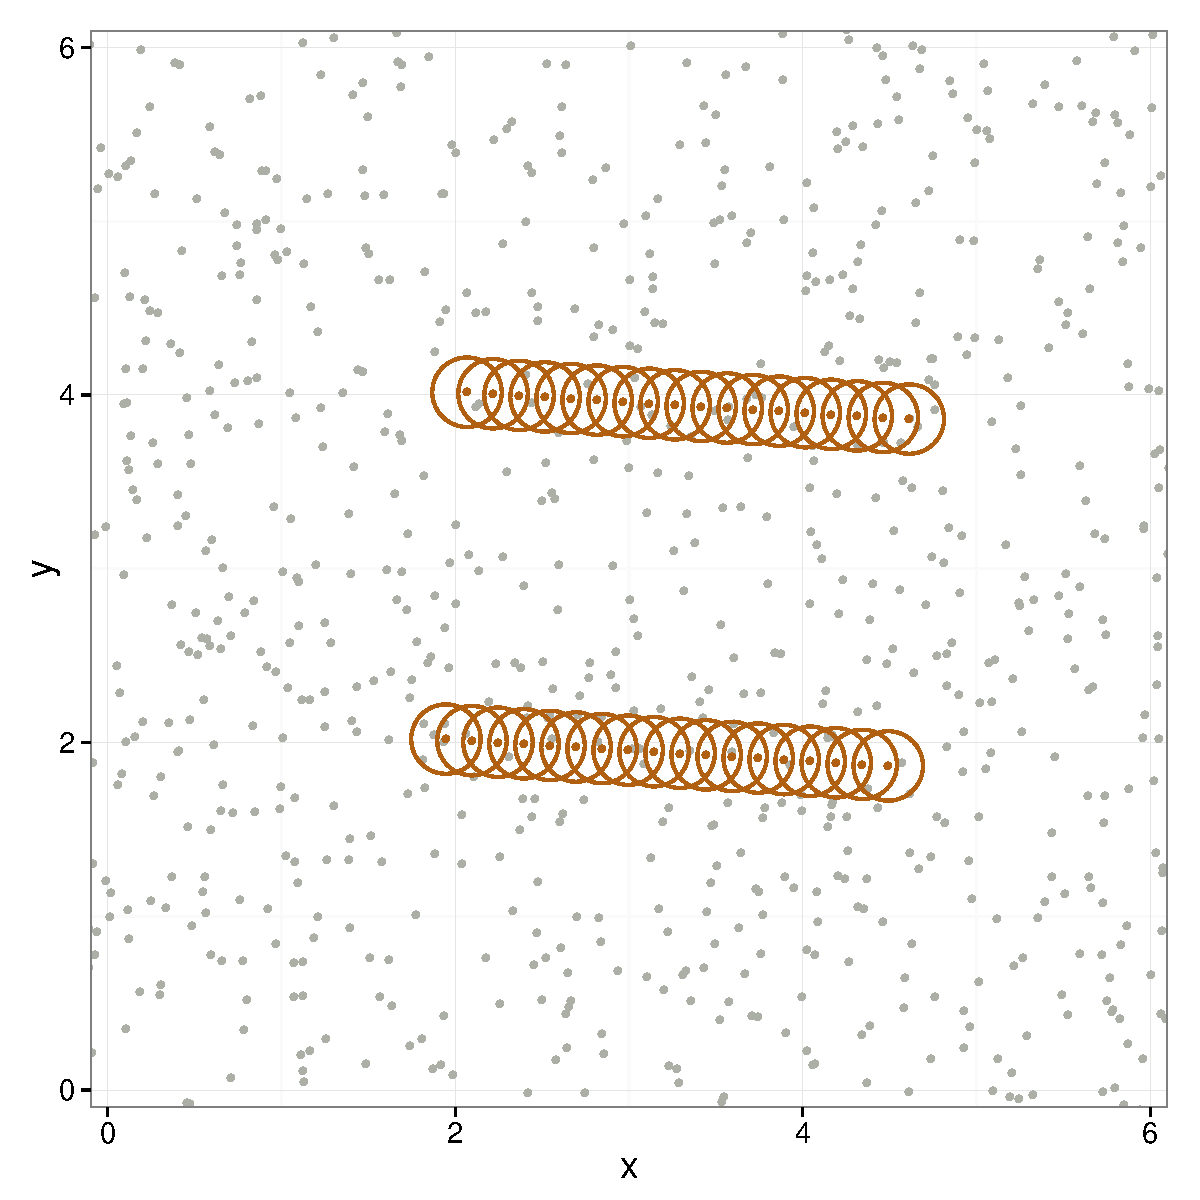
\includegraphics[width=\textwidth]{../images/slides-layoutT1.pdf}
		\end{column}
	\end{columns}

	\note{
	\begin{itemize}
	\item 2 transects, 18 stations each
	\item angle randomly chosen
	\item starting position randomly chosen
	\end{itemize}	
	}
\end{frame}

\begin{frame}{Structured and Random Layouts}
Examples of Structured and Random layouts.\\
1 unit on graph = 1 km
	\begin{columns}
		\begin{column}{0.48\textwidth}
			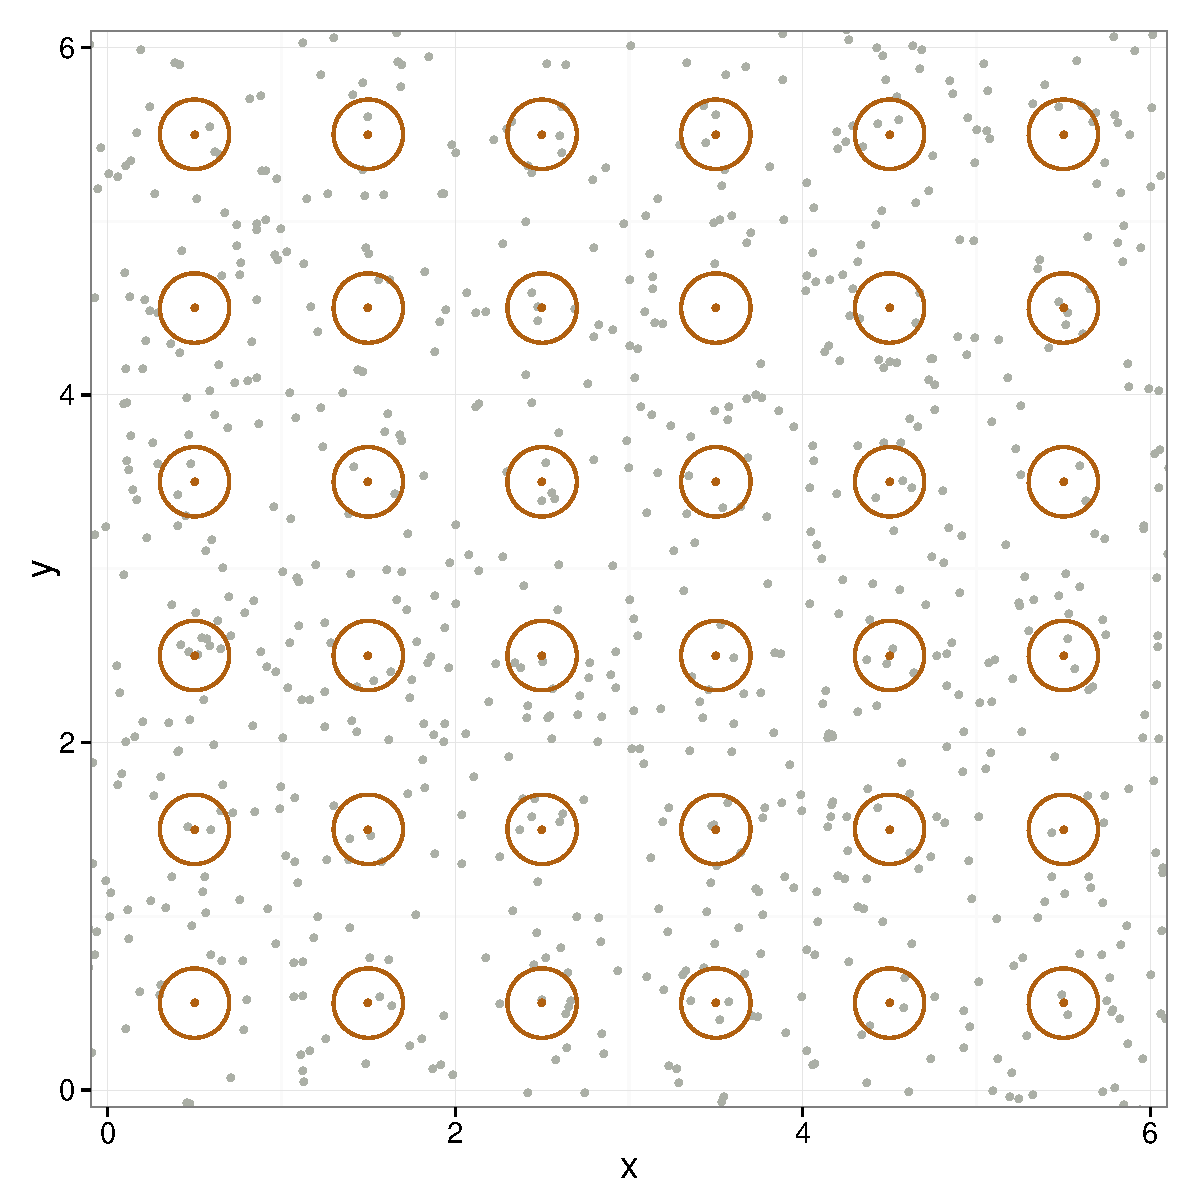
\includegraphics[width=\textwidth]{../images/slides-layoutS.pdf}
		\end{column}
		\begin{column}{0.48\textwidth}
			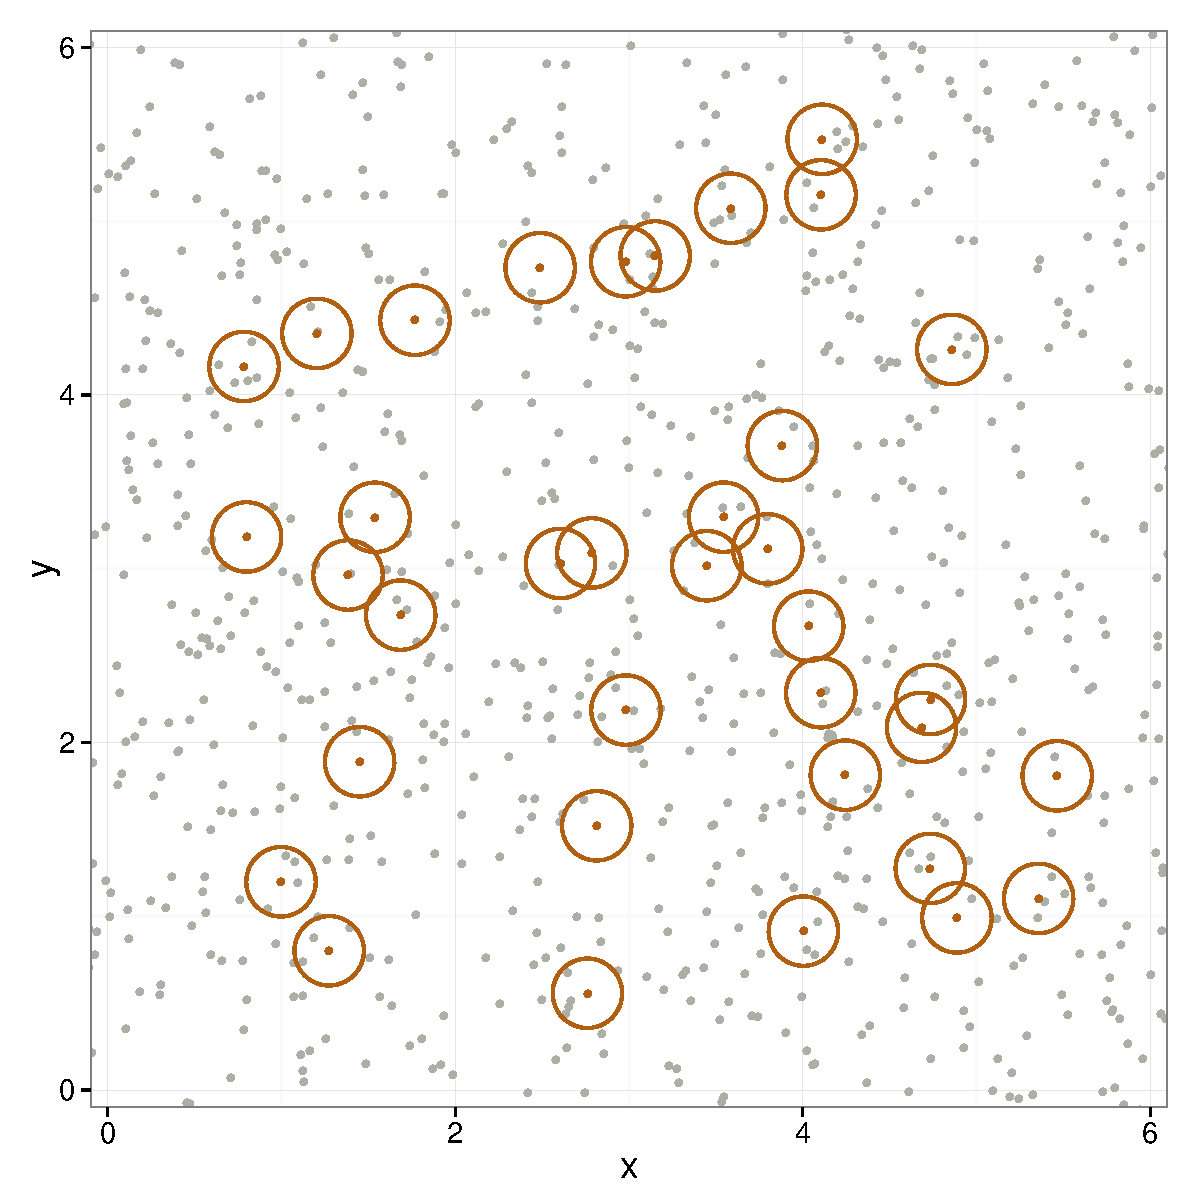
\includegraphics[width=\textwidth]{../images/slides-layoutR.pdf}
		\end{column}
	\end{columns}

	\note{
		\begin{itemize}
		\item Structured layout is why we're at 6km$^2$. needed to be able to have 500 m of direction in either area, without overlap
		\item this gave 36 stations, which was carried over to the other layout types.
		\item For Random Method, center point of VCP was randomly placed, within the buffer zone.
		\end{itemize}	
	}
\end{frame}

\begin{frame}{Detection Curve: Ideal}
``Ideal'' detection probability curve, maximum observation distance set to 0.5 unit (500 m) distance, and scaled so $g(0)=1$
	\begin{figure}
		\centering
		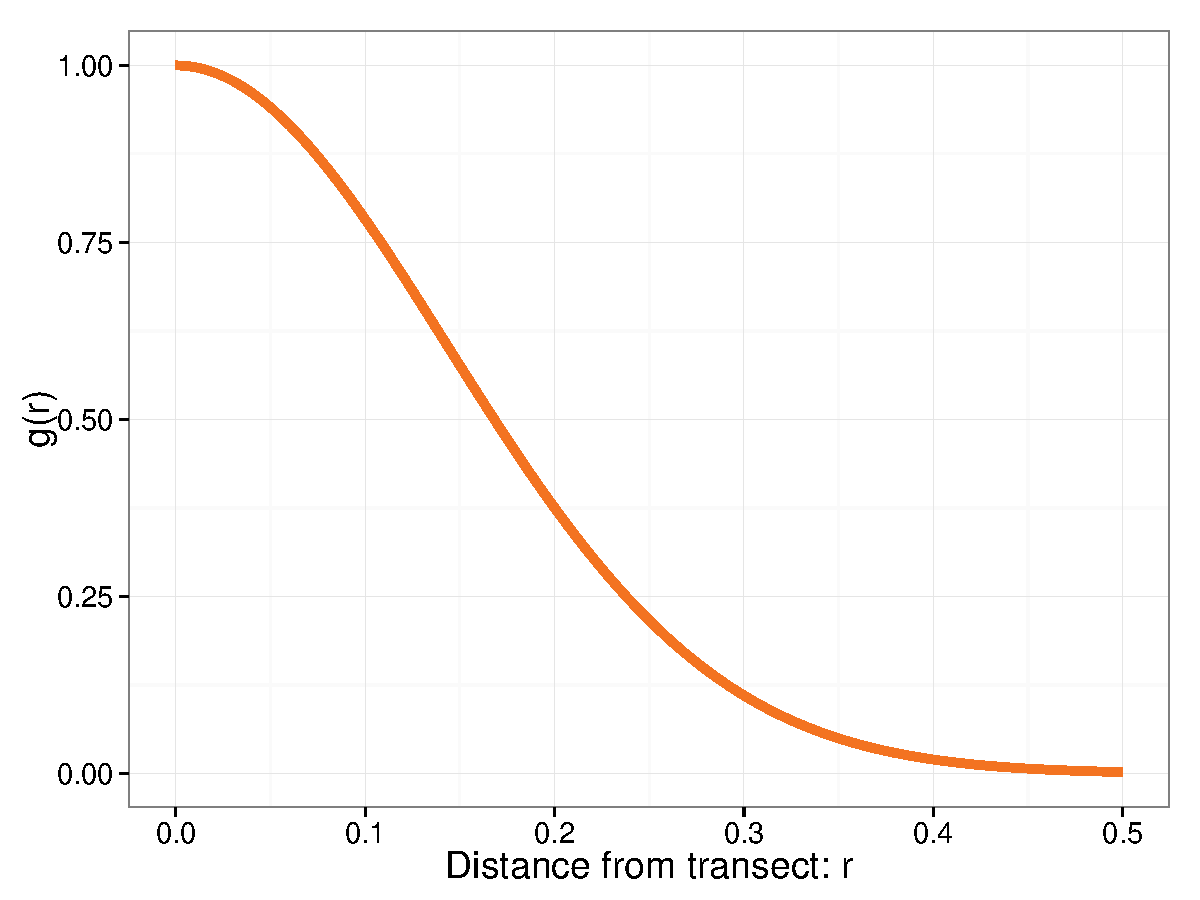
\includegraphics[height=.75\textheight]{../images/detectionCurveScaled.pdf}
	\end{figure}
		\note{
			\begin{itemize}
			\item A halfnormal curve, scaled so that $g(0.5)~0$ and $g(0)=1$
			\item used FDRTOOL package in R.
			\end{itemize}	
		}
\end{frame}

\begin{frame}{Detection Curve: Empirical}
Detection probability curve from empirical data, shown unscaled.
	\begin{figure}
		\centering
		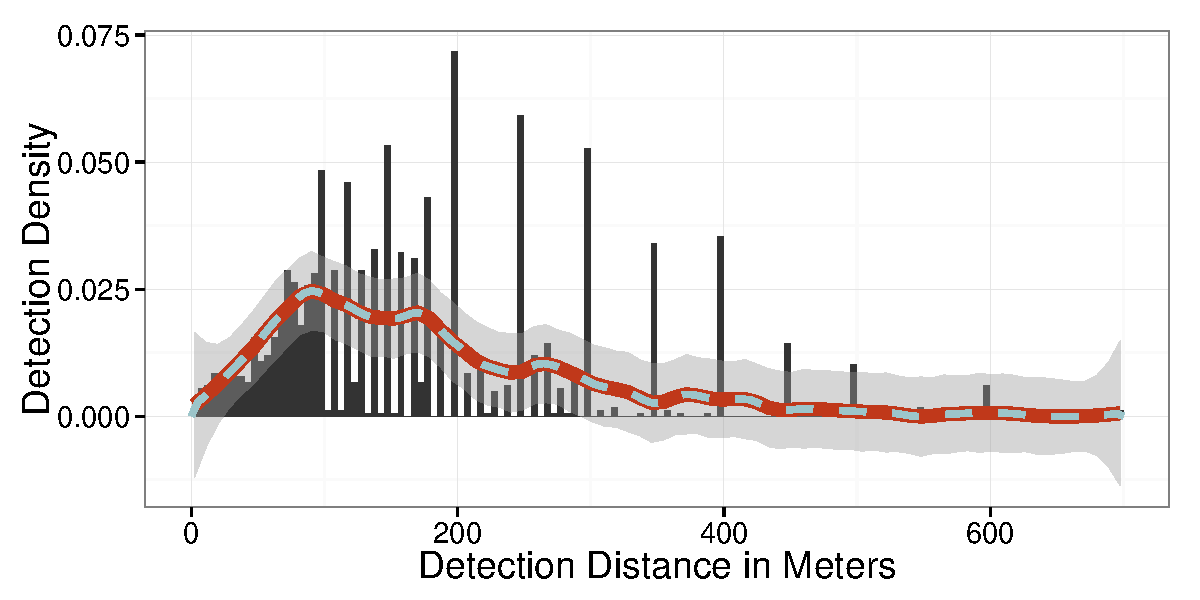
\includegraphics[width=\textwidth]{../images/loess.pdf}
	\end{figure}
	
		\note{
			\begin{itemize}
			\item data heaped into 5 m bins, midpoint of bin as x, density of bin * 5 as y
			\item Loess regression performed with a span of 2. This is solid line.
			\item Gives us object that can be used with predict function. Dashed line is estimate run with Predict to ensure.
			\item As with the half-normal, the density was scaled so that the highest point gave a probability of 1.
			\item with Predict, distances that extrapolated beyond the original dataset returned ``na'', these were set to a probability of detection of 0.
			\end{itemize}	
		}
\end{frame}

\begin{frame}{Movement}
	The histogram of observed distances shows evidence of movement, so it was considered as an option for simulation.\\
	\vspace{0.33cm}
	Three Movement Options:
	\begin{itemize}
	\item No Movement: Objects stayed at origin point
	\item[]
	\item Temporary Movement: Objects would shift away from observer, but shift back to origin after observer ``left''
	\item[]
	\item Compounded Movement: Objects would shift away from observer, would remain at new point after observer moved. (Movement could compound if object was within movement radius for more than one VCP)
	\end{itemize}
	
	\note{
		\begin{itemize}
		\item Based on the empirical observations, movement was simulated within the first 100 m from observer
		\item Higher chance of movement if closer to observer
		\item Moved further if originated closer to observer.
		\end{itemize}	
	}
\end{frame}
% -------------------------------- RESULTS --------------------------------------------------
\section{Results}

\begin{frame}{Empirical vs. Half-Normal}
	\small
	1000 simulations, comparing Empirical vs Half-Normal detection probability, no movement, 
	\begin{figure}
		\centering
		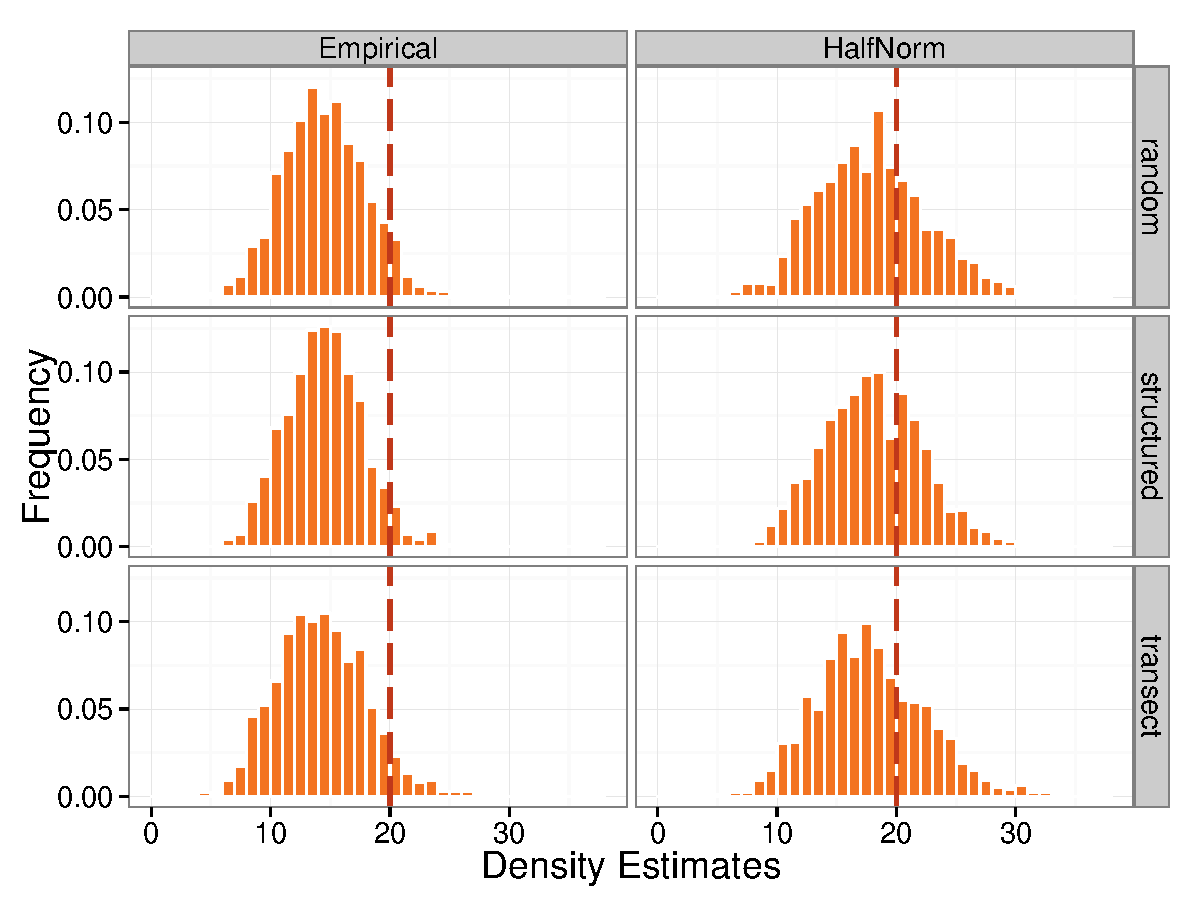
\includegraphics[height=.80\textheight]{../images/Emp_Vs_Hnorm_1-2.pdf}
	\end{figure}
	\note{
		\begin{itemize}
		\item 1000 Simulations. Each object layout was analyzed with the 6 combinations represented in the graph
		\item Density estimates done using the kernel method with a normal kernel \parencite{quang1993}
		\item Estimates for Empirical detection function biased low.
		\item Estimates using half-normal detection function biased low, but not as bad.
		\end{itemize}	
	}

\end{frame}


\begin{frame}{Empirical vs. Half-Normal}{Centers and Spread}

\begin{table}
	\begin{tabular}{ r r |r r| r r r}
		$g(x)$      & Layout     & Mean  & Std Dev & 25th  & Median & 75th  \\ \hline\hline
		Empirical   & Random     & 14.47 & 3.37    & 12.08 & 14.38  & 16.73 \\
		Empirical   & Structured & 14.49 & 3.15    & 12.27 & 14.47  & 16.59 \\
		Empirical   & Transect   & 14.26 & 3.66    & 11.65 & 14.14  & 16.80 \\ \hline
		Half-normal & Random     & 17.90 & 4.57    & 14.67 & 17.86  & 20.88 \\
		Half-normal & Structured & 18.03 & 4.16    & 15.05 & 17.91  & 20.82 \\
		Half-normal & Transect   & 17.80 & 4.64    & 14.52 & 17.44  & 20.78
	\end{tabular}
\end{table}
\small
Comparing measures of centers and spread, 1000 simulations, no movement.

	\note{
	\begin{itemize}
	\item supports graphic: Centers vary between detectability options, but not much between layouts.
	\item May be some evidence of a downward shift with the Transect Layout. Can observe in Empirical mean \& median, and Half-normal Median. 
	\item Hard to say if this is true effect or something else.
	\end{itemize}
	}
\end{frame}

\begin{frame}{Empirical vs. Half-Normal}{True Density Capture}
\begin{table}

	\begin{tabular}{ r| r r| r r|}
		           & \multicolumn{2}{|c|}{Empirical} & \multicolumn{2}{|c|}{Half Normal} \\ \hline\hline
		Layout     & Mean $\hat{D}$ & \% Capture     & Mean $\hat{D}$ & \% Capture       \\ \hline\hline
		Random     & 14.47          & 73.6\%         & 17.90          & 94.0\%           \\
		Structured & 14.49          & 77.5\%         & 18.03          & 95.3\%           \\
		Transect   & 14.27          & 69.6\%         & 17.80          & 91.2\%           \\ \hline
	\end{tabular}

\end{table}

\small
Comparing rates of capture for true object density, 1000 simulations, no movement.

	\note{
	\begin{itemize}
	\item Again, Transect layout may have some downward trend, as the capture percentages are lower here
	\item Everything is relative. We have a larger up-tick in the Empirical/Structured cell than for Half-Normal and Structured.
	\item Repeated runs of the simulation, and higher simulation counts could help determine if this is a significant pattern.
	\end{itemize}
	}
\end{frame}

\begin{frame}{Movement Results}
\small
	1000 simulations, comparing effect of movement types. Half-normal detection probability used for all.
	\begin{figure}
		\centering
		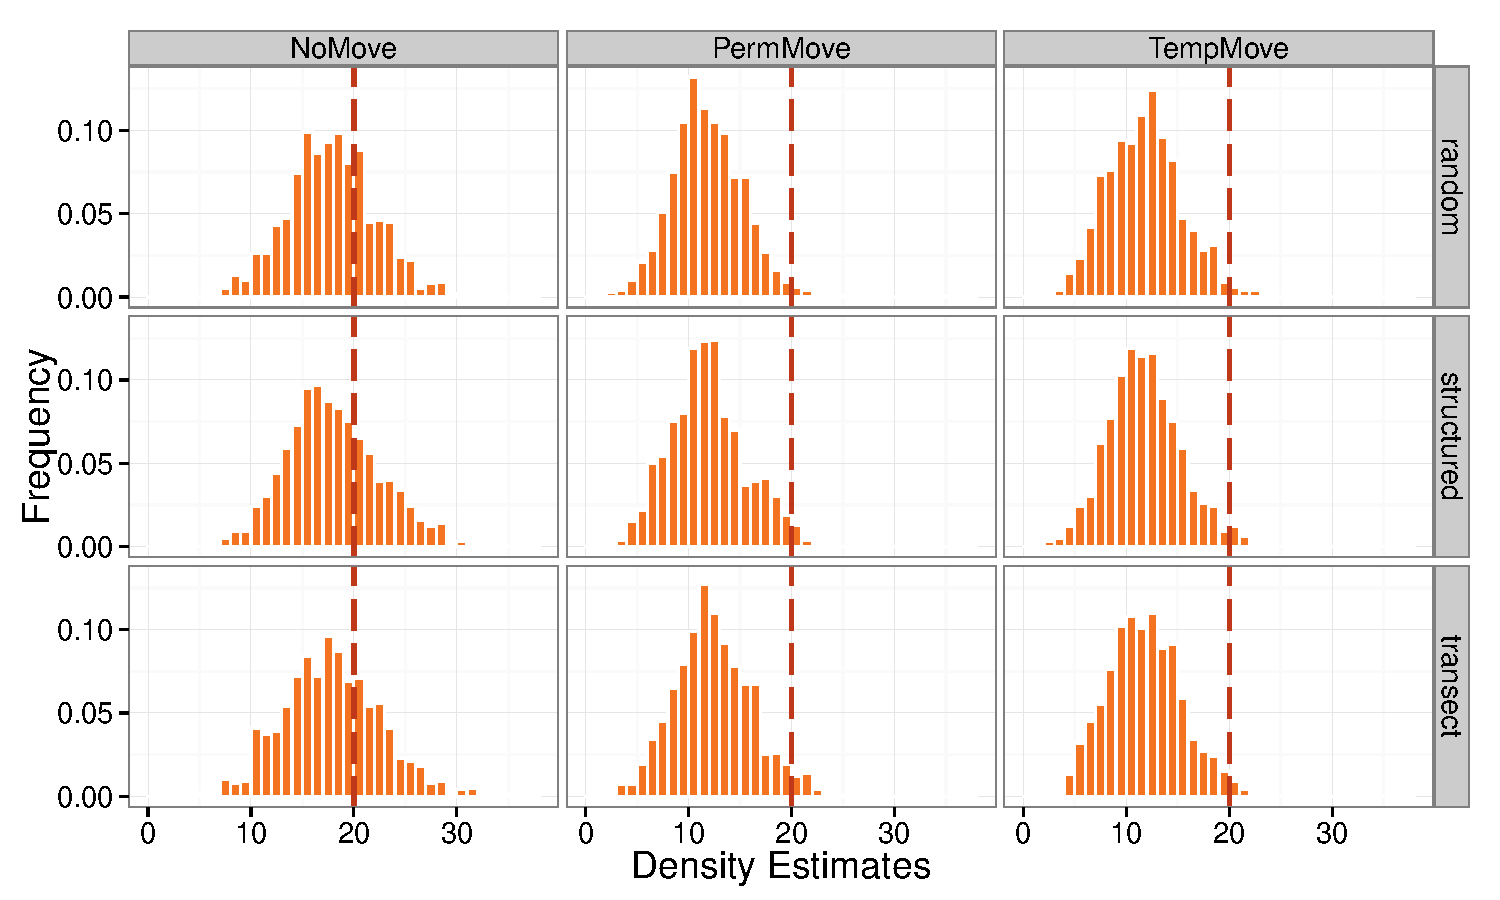
\includegraphics[height=.80\textheight]{../images/MovementSim2.pdf}
	\end{figure}
	\note{
		\begin{itemize}
		\item 1000 Simulations. Again, each object layout was analyzed with the 9 combinations represented in the graph
		\item Density estimates done using the kernel method with a normal kernel \parencite{quang1993}
		\item Again, layout does not seem to play as large of a part as the other factor.
		\item All were run with half-normal detectability function
		\end{itemize}	
	}
\end{frame}

\begin{frame}{Movement Results}{Centers \& Spread}

	\begin{table}
	
		\begin{tabular}{ r r| r r| r r r}
			Movement  & Layout     & Mean  & Std Dev & 25th  & Median & 75th  \\ \hline\hline
			None      & Random     & 17.86 & 4.28    & 15.03 & 17.64  & 20.65 \\
			None      & Structured & 18.01 & 4.51    & 14.95 & 17.62  & 20.94 \\
			None      & Transect   & 17.90 & 4.78    & 14.74 & 17.67  & 20.95 \\ \hline
			Compounded & Random     & 11.86 & 3.42    & 9.58  & 11.61  & 14.09 \\
			Compounded & Structured & 11.90 & 3.65    & 9.37  & 11.67  & 14.08 \\
			Compounded & Transect   & 12.42 & 3.72    & 9.93  & 12.17  & 14.79 \\ \hline
			Temporary & Random     & 11.76 & 3.57    & 9.22  & 11.75  & 14.02 \\
			Temporary & Structured & 11.74 & 3.48    & 9.37  & 11.56  & 13.85 \\
			Temporary & Transect   & 11.75 & 3.57    & 9.24  & 11.72  & 14.20
		\end{tabular}
	\small
	Comparing measures of center and spread for different movement types. 1000 simulations, half-normal detection probability used for all.
	\end{table}
	\note{
	\begin{itemize}
	\item Reinforced histograms: results consistent within movement type, regardless of layout type
	\item No Movement is consistent with what was observed in initial simulation
	\item 
	\end{itemize}
	}
\end{frame}

\begin{frame}{Movement Results}{True Density Capture}

	\begin{table}
	
		\begin{tabular}{ r| c c| c c| c c|}
		
			& \multicolumn{2}{|c|}{No Movement}	& \multicolumn{2}{|c|}{Compounded}	& \multicolumn{2}{|c|}{Temporary}\\ 
	 \hline \hline
	
	 Layout		&\footnotesize Mean $\hat{D}$	&\footnotesize \%  &\footnotesize Mean $\hat{D}$ &\footnotesize \%  &\footnotesize Mean $\hat{D}$ &\footnotesize \% 	\\ \hline \hline
	 Random		& 17.86 			& 94.2\% 		& 11.86	& 59.6\%	& 11.76	& 59.3\% \\
	 Structured	& 18.01 			& 94.3\% 		& 11.90 & 59.9\% 	& 11.74 & 59.5\% \\
	 Transect	& 17.90 			& 90.8\% 		& 12.42 & 65.0\% 	& 11.75 & 58.0\% \\ \hline
	
		\end{tabular}
	
	\end{table}
	\small
	Comparing capture of true object density for different movement types. 1000 simulations, half-normal detection probability used for all.
	\note{
	\begin{itemize}
	\item Movement type does not appear to play a large part in changing the bias.
	\item We capture the true density about 59\% of the time, regardless of movement type.
	\end{itemize}
	}
\end{frame}

\begin{frame}{Movement And Layouts}
	
	\begin{columns}
		\begin{column}{0.3\textwidth}
			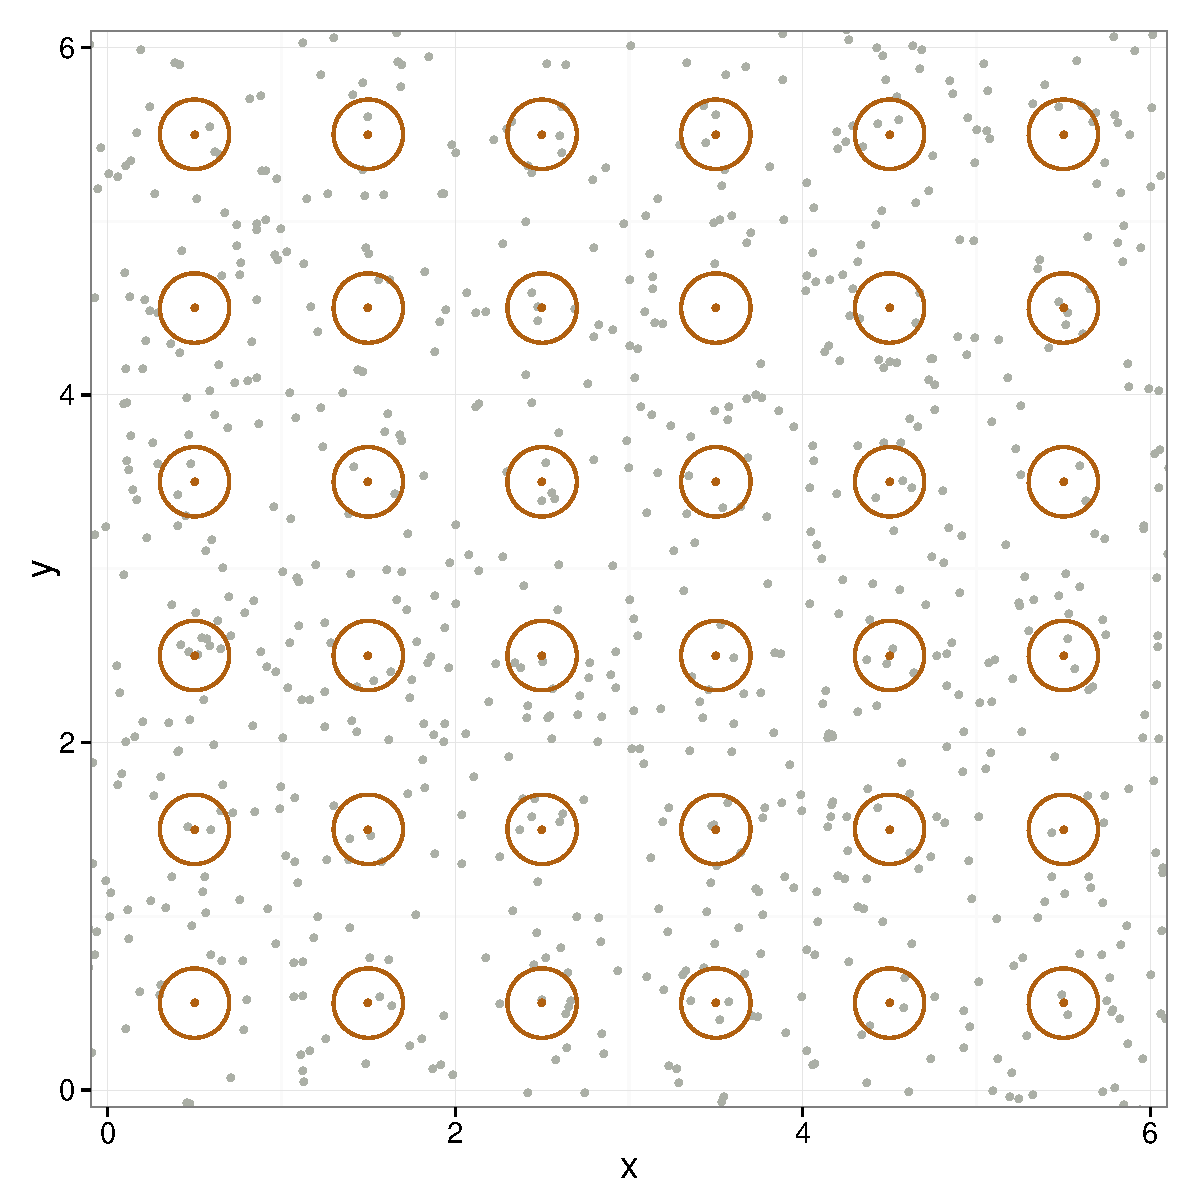
\includegraphics[width=\textwidth]{../images/slides-layoutS.pdf}
		\end{column}
		\begin{column}{0.3\textwidth}
			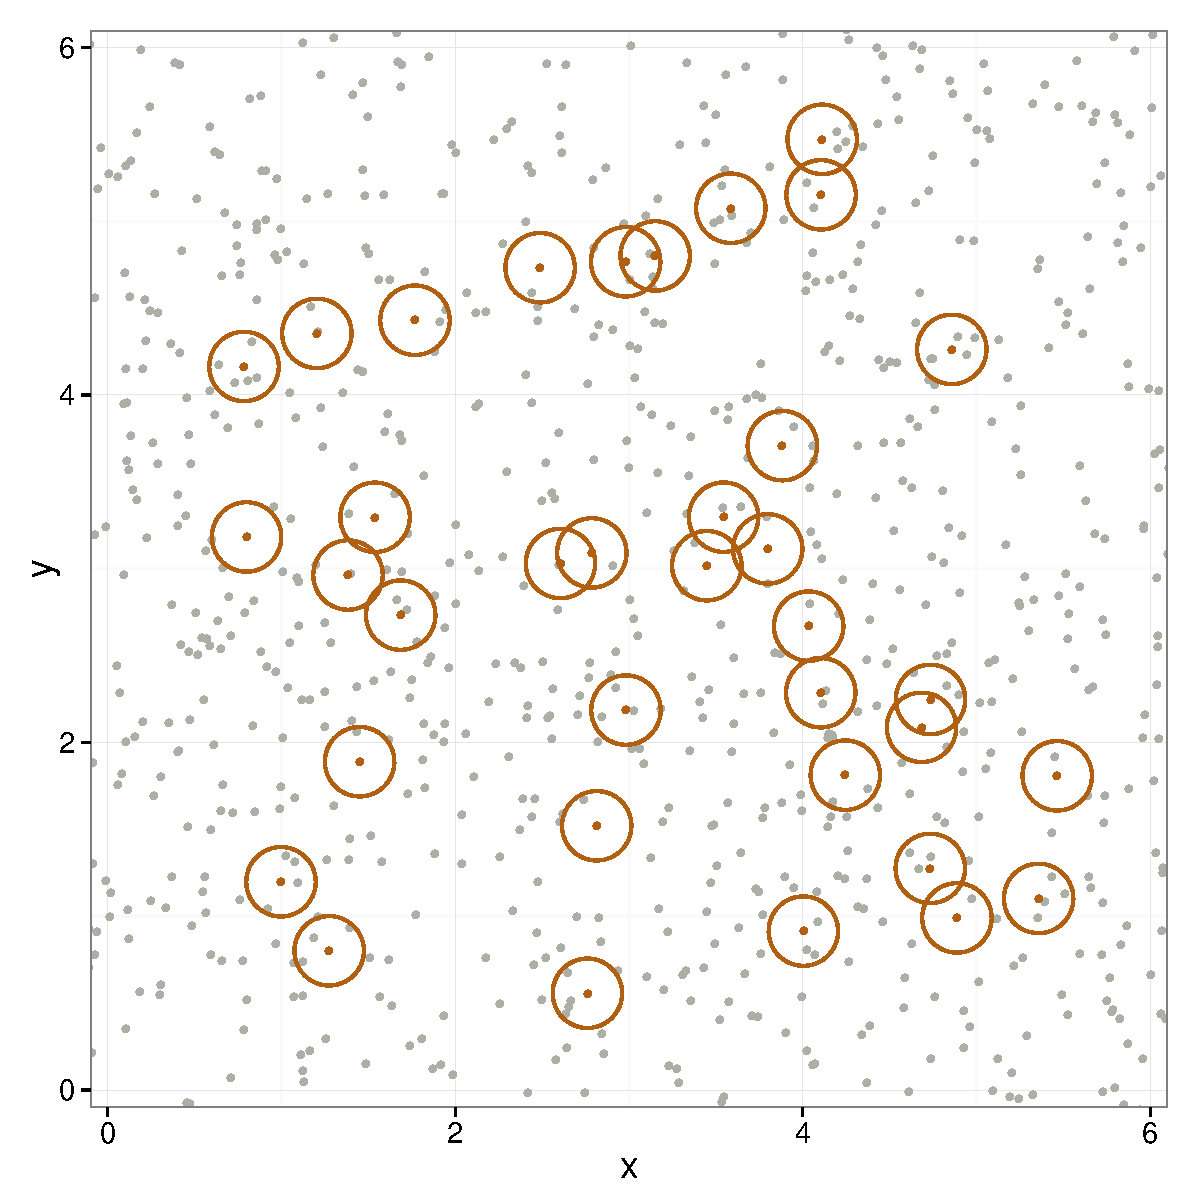
\includegraphics[width=\textwidth]{../images/slides-layoutR.pdf}
		\end{column}
		\begin{column}{0.3\textwidth}
			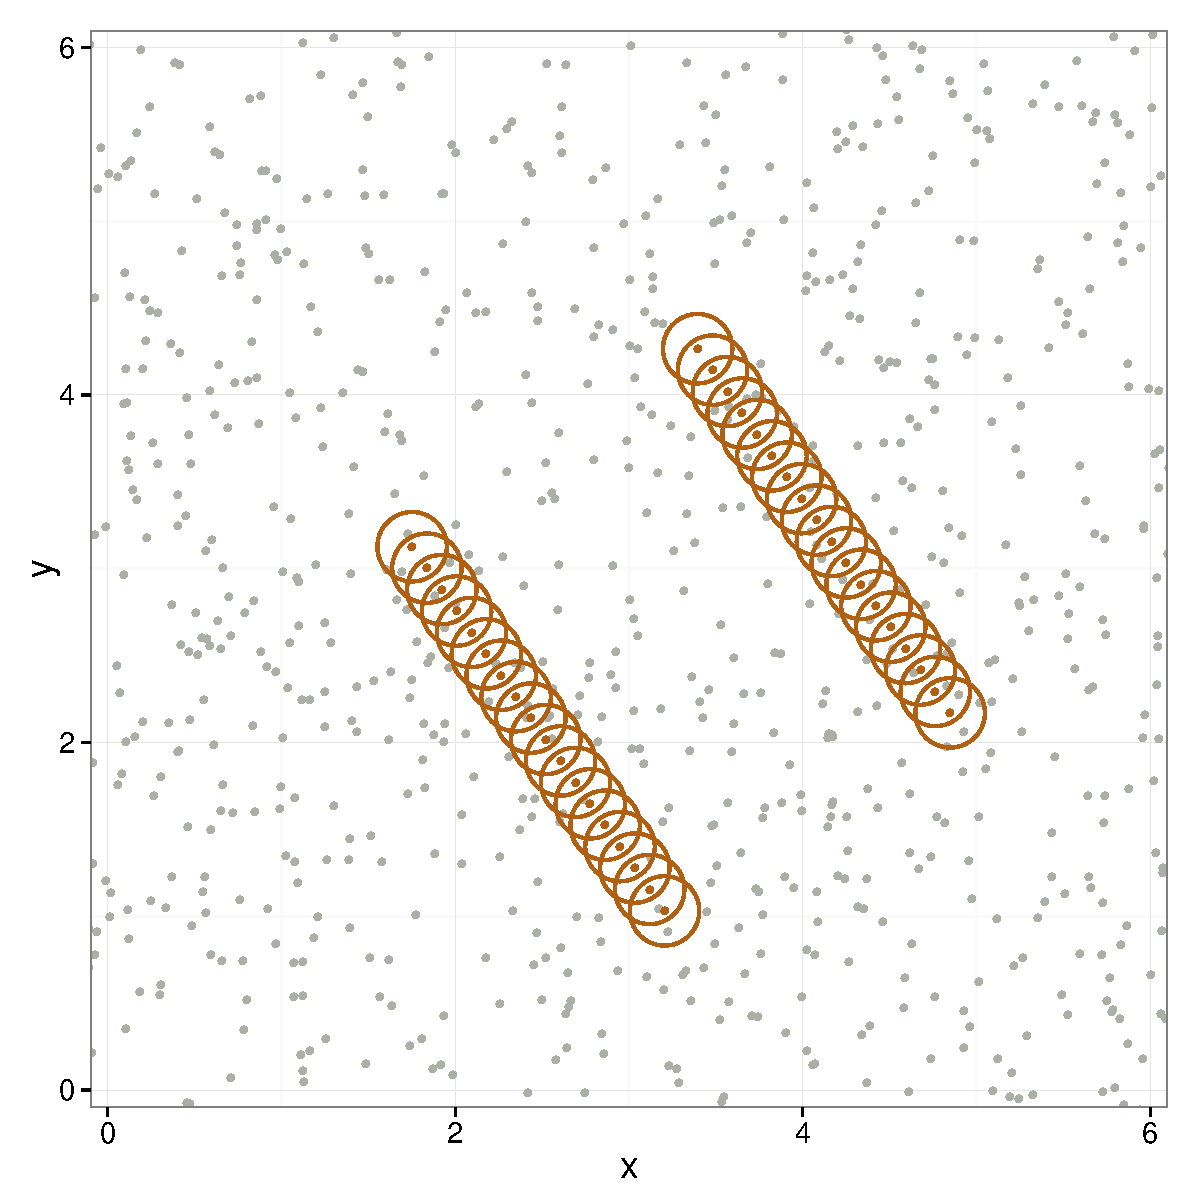
\includegraphics[width=\textwidth]{../images/slides-layoutT2.pdf}
		\end{column}
	\end{columns}
	\vspace{1cm}
	1 unit = 1 km, circles represent 200 m out from station
	\note{
		\begin{itemize}
		\item Makes sense for structured, if the objects are only moving within the first 100 m, they would not move twice.
		\item For the Randomized Layout, there are only 3, in this example, where there is a significant amount of overlap. If we take this as representative of the population of layouts, we would not be seeing many layouts with a significant amount of double or triple movement. An estimate from this layout should be similar to the Structured Layout, which we see.
		\item It's with the Transect layout where the most compounded movement occurs.
		\item (Go Back 1 Slide) There may be an effect of the combination of The Compounded movement and the Transect layout.
		\item not sure if this is bias reduction, or an upward bias that looks like bias reduction because we're already low.
		\end{itemize}
	}
\end{frame}



% -------------------------------- Lines vs. Circles --------------------------------------------------
\section{Problems}

\begin{frame}{Movement Testing}
Results of movement code test (left) vs no movement ``baseline'' (right).
	\begin{figure}
		\centering
		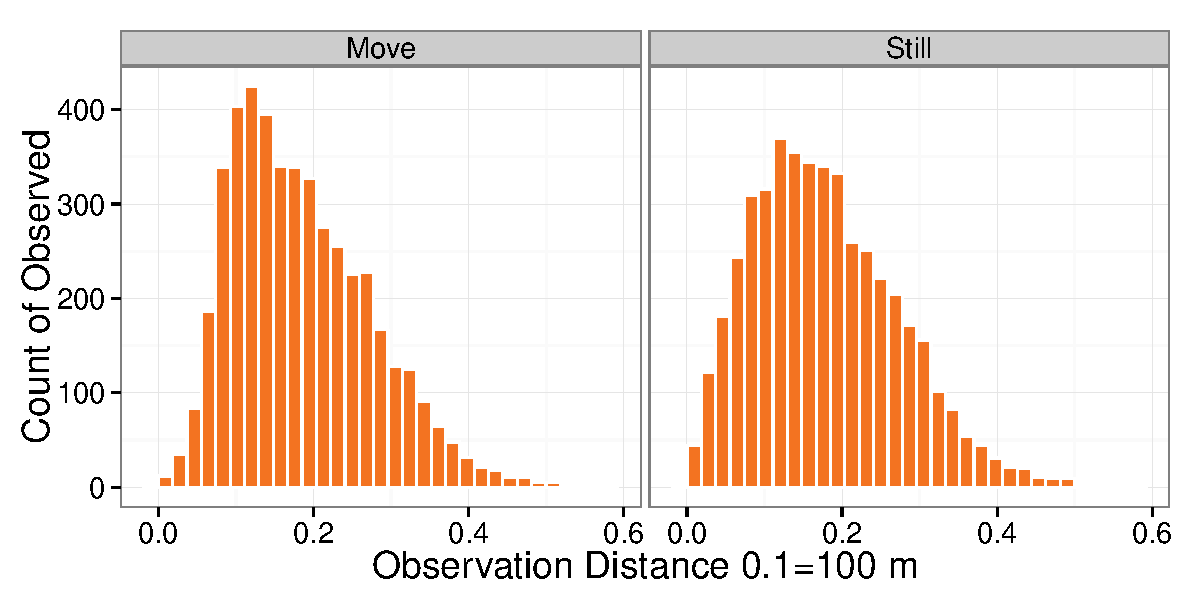
\includegraphics[width=\textwidth]{../images/movementTest.pdf}
	\end{figure}
\end{frame}

\begin{frame}{Change in Area}
	Area increase from 1 unit expansion in Line Transect does not equal the area from the same increase in a VCP.
	\begin{columns}
		\begin{column}{0.48\textwidth}
		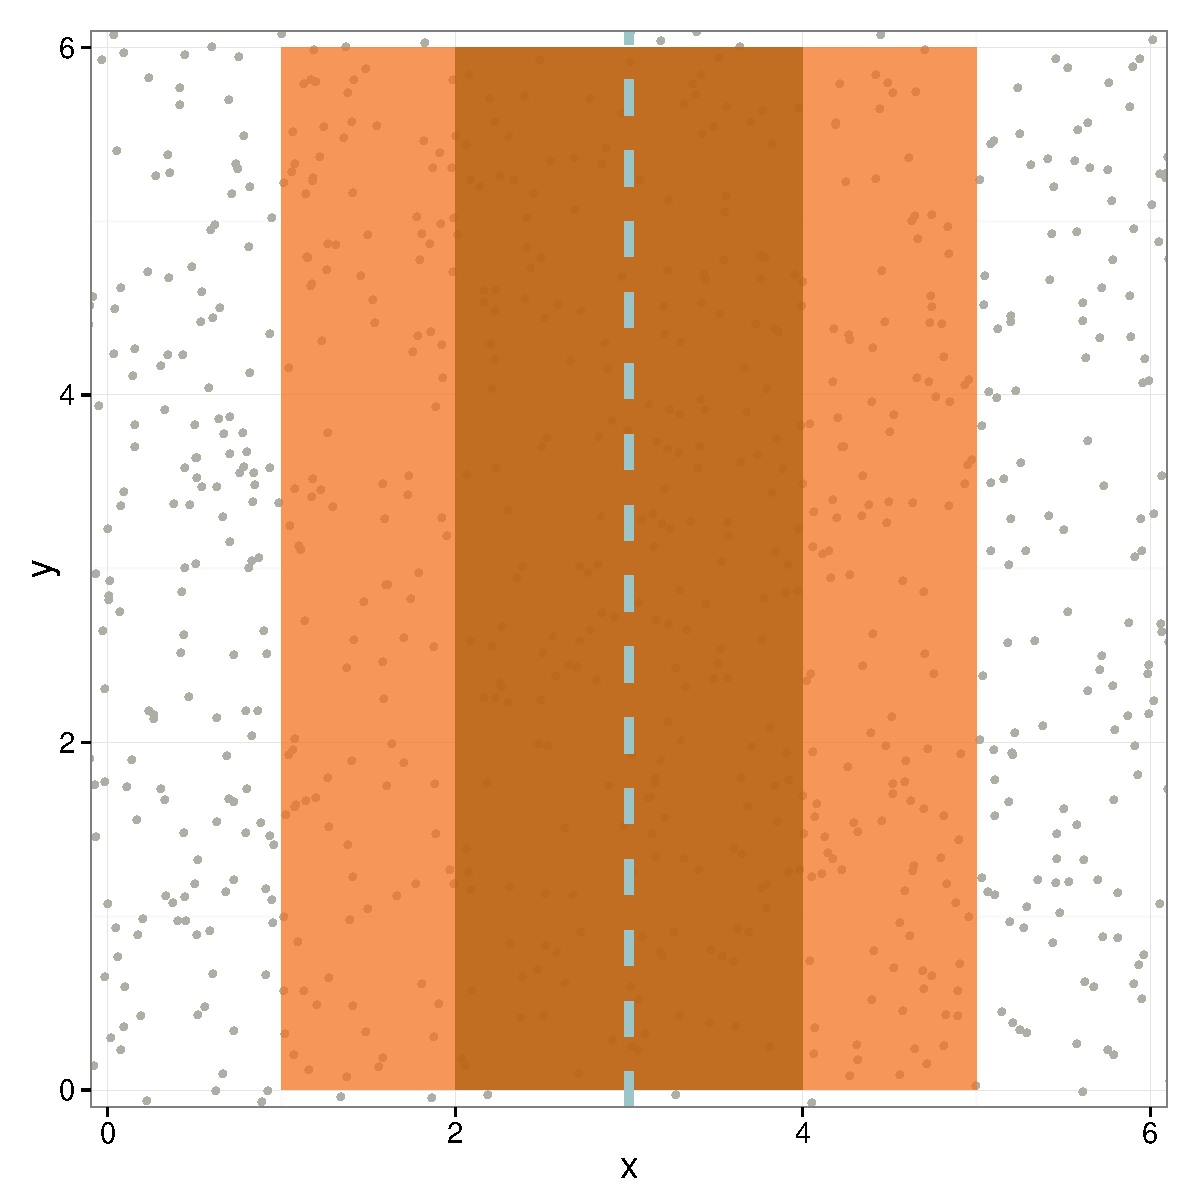
\includegraphics[width=\textwidth]{../images/slides-LTr.pdf}
		\end{column}
		\begin{column}{0.48\textwidth}
		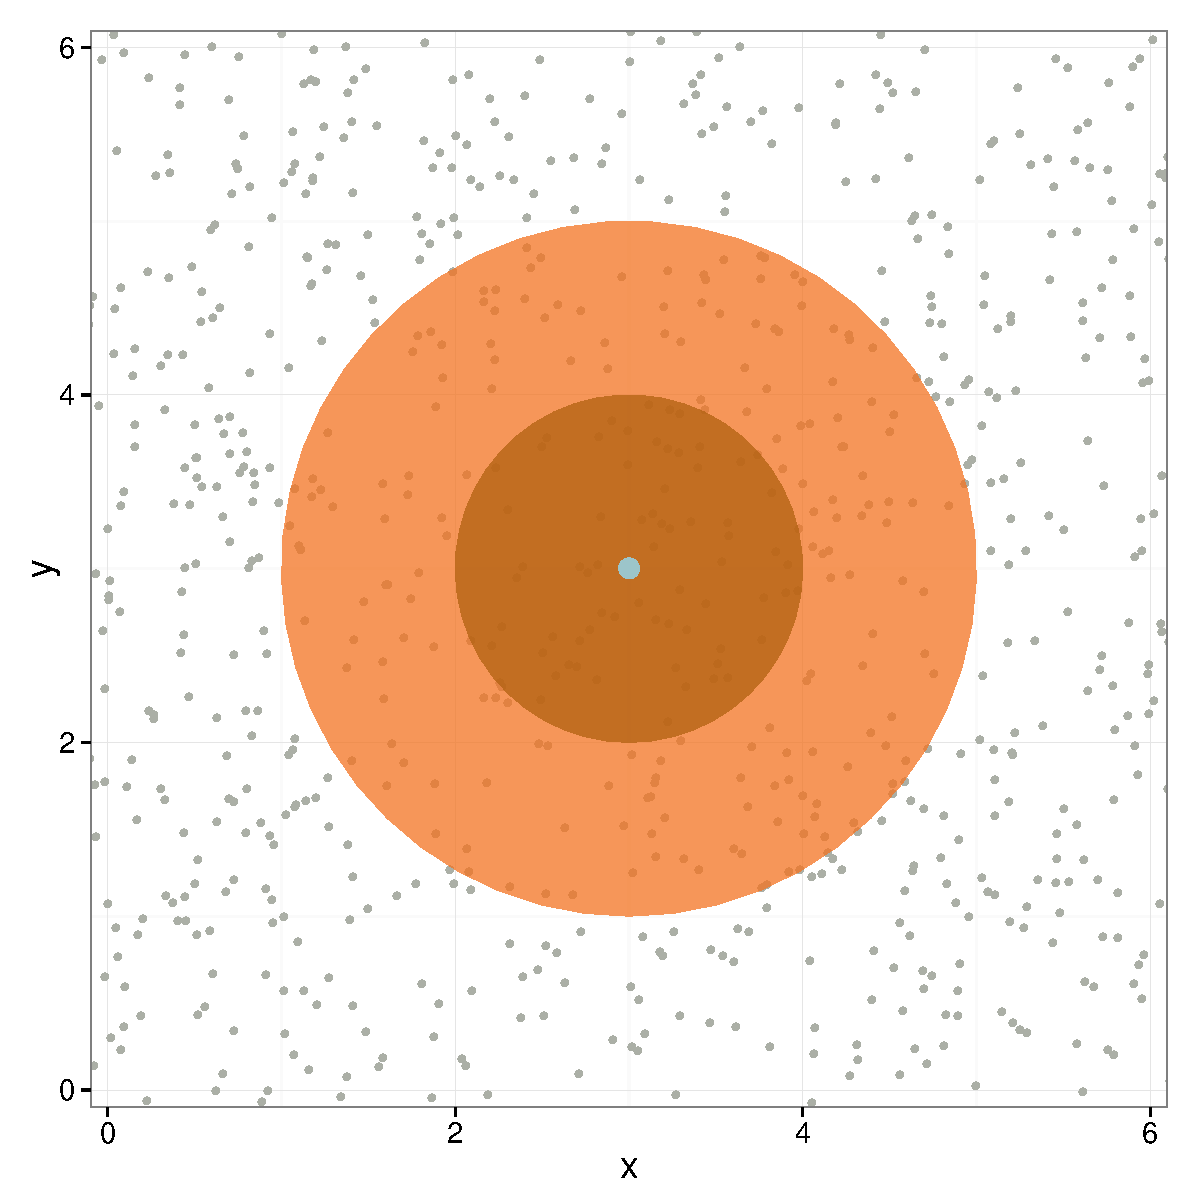
\includegraphics[width=\textwidth]{../images/slides-VCPr.pdf}
		\end{column}
	\end{columns}

\end{frame}

\begin{frame}{Circles vs. Rectangles}{Area and Expected Observation Counts}
	\begin{columns}
		\begin{column}{0.48\textwidth}
		\centering
		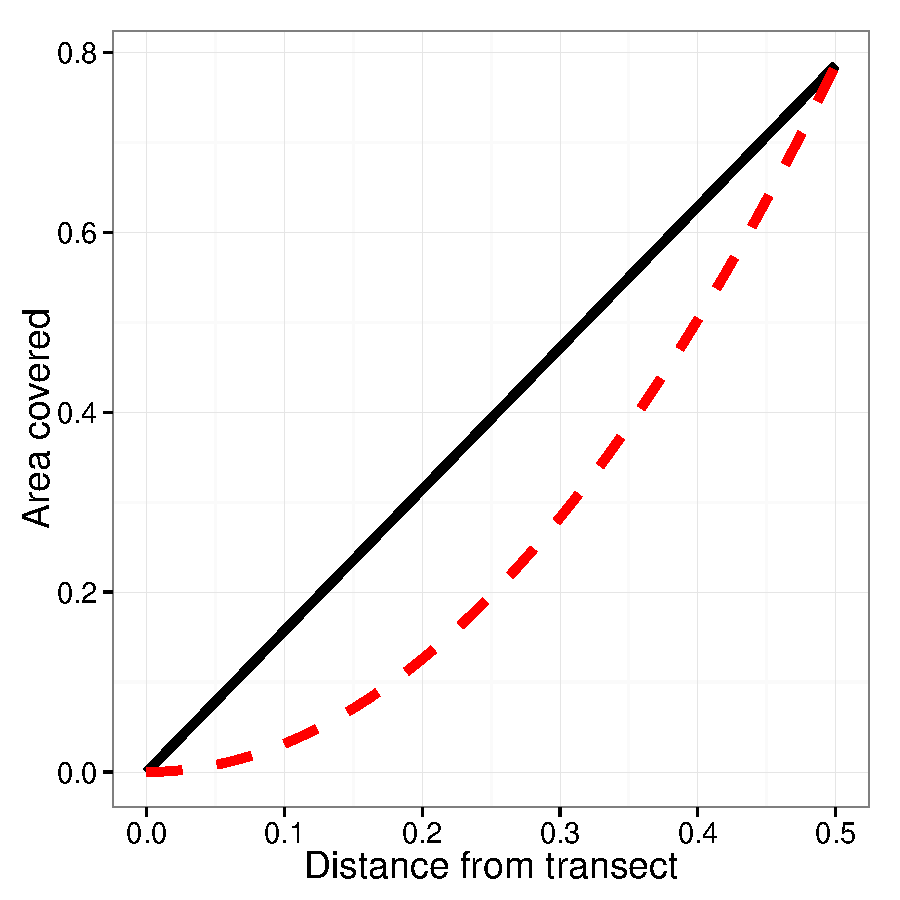
\includegraphics[width=\textwidth]{../images/rect-circ-area.pdf}\\
		\small
		Increase in Area
		\end{column}
		\begin{column}{0.48\textwidth}
		\centering
		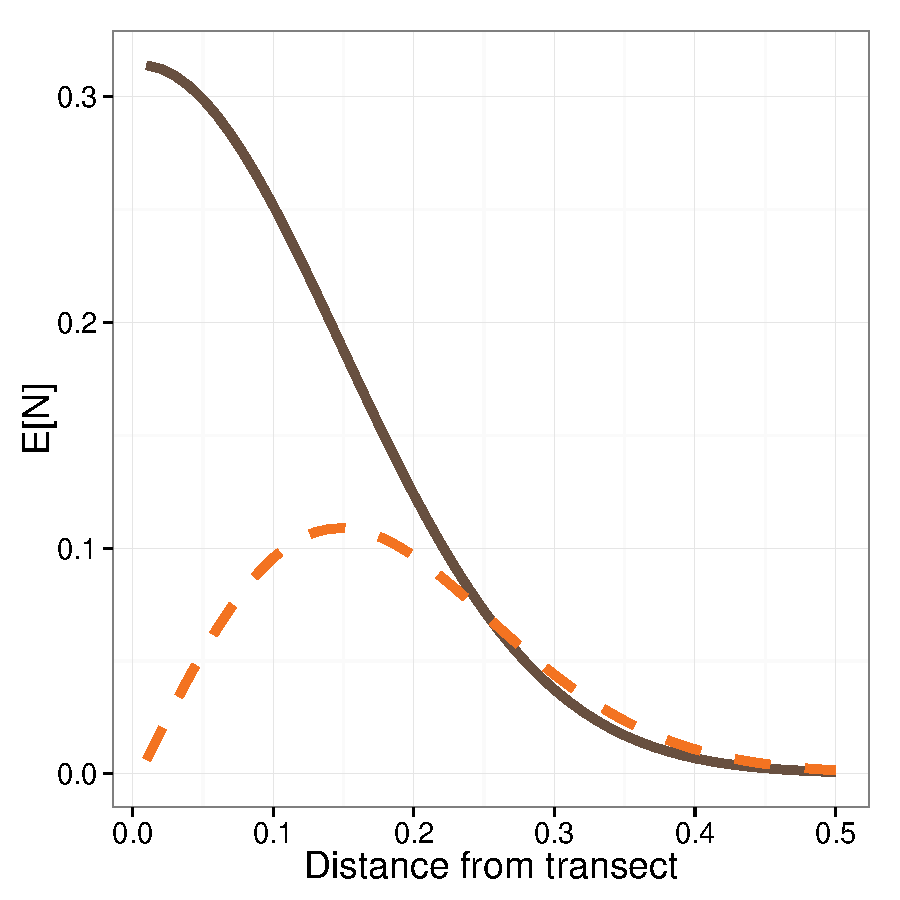
\includegraphics[width=\textwidth]{../images/rect-circ-detection.pdf}\\
		\small
		Expected number of observations, given distance.
		\end{column}
	\end{columns}
	\begin{center}
	\par Solid line is Line Transect, Dashed line is VCP
	\end{center}
	
\end{frame}


% -------------------------------- CONCLUSION --------------------------------------------------
\section{Conclusion}

\begin{frame}{Conclusion}
There are two primary conclusions:\\
\vspace{0.5cm}
	\begin{itemize}
	\item If all else is held equal, VCP layout does not seem to play a large role in the bias of population density estimates using the kernel method described by \textcite{quang1993}.
	\item[]
	\item Violations of the expected detection probability curve, or by movement of the objects away from the observer play a greater role in biasing the resulting estimate.
	\end{itemize}

	
	\note{
	\begin{itemize}
	\item All of the estimates were biased low using Quang's formula
	\item this was observed even with an ``ideal'' half-normal detection curve
	\item Dr. Quang's paper does offer a bias-corrected estimate, but it was not used for this project.
	\end{itemize}
	}
\end{frame}

\begin{frame}{Future Work}
Some possible areas for future research:

	\begin{itemize}
	\item Explore the possible interaction effect from Compounded Movement and the Transect Layout
	\item[]
	\item Modify simulation functions to return more information to assist diagnostics
	\begin{itemize}
	\item Count of Observed Objects
	\item Observation Distances
	\end{itemize}
	\item[]
	\item Modify using the Empirical data as a detectability function, to account for difference between line and point transects.
	\end{itemize}
\end{frame}

\begin{frame}{Future Work}
	\begin{itemize}
	\item Add the option to bias-correct the estimates, to see how well Quang's kernel method adjusts for these variations.
	\item[]
	\item Address analyzing transects as clusters, since observations on a transect are likely to be related.

	\end{itemize}
\end{frame}

\begin{frame}{Final Words}
	\begin{quote}
	``All models are wrong, but some are useful.'' --George E. P. Box
	\end{quote}
\end{frame}

	\begin{frame}{Acknowledgements}
	Micronesian Survey Data courtesy of Fred Ramsey\\
	\vspace{1cm}
	Masters Committee:
	\begin{itemize}
	\item[] Claudio Fuentes, Advisor
	\item[] Alix Gitelman, Committee Member
	\item[] Charlotte Wickham, Committee Member
	\end{itemize}
\end{frame}




\begin{frame}{Questions? }
	\begin{figure}
		\centering
		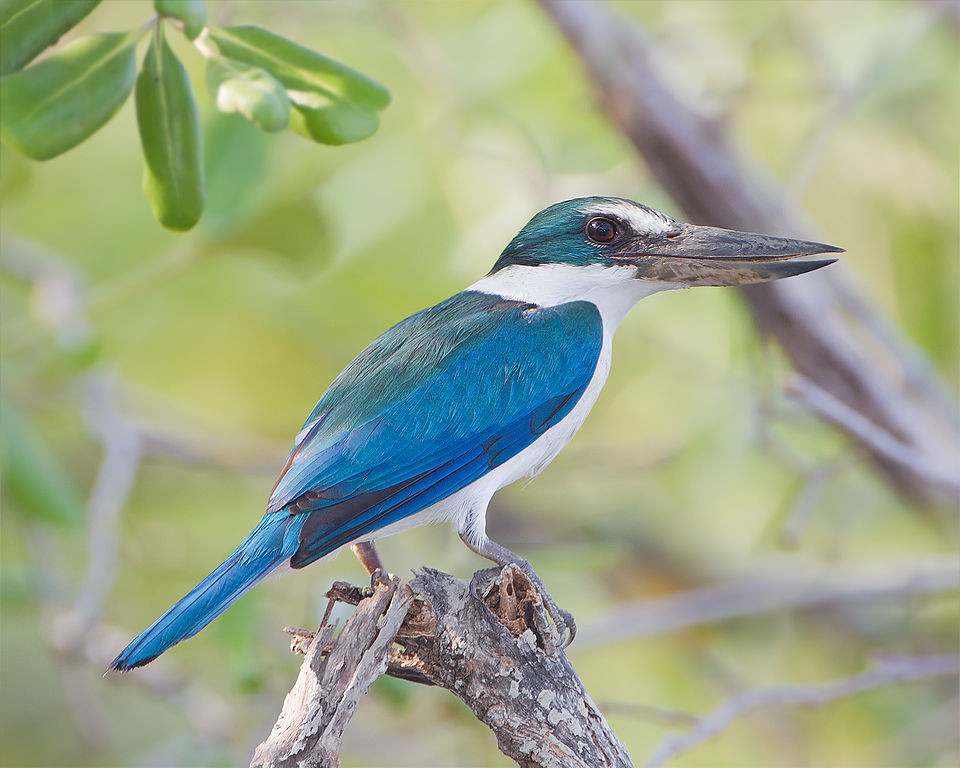
\includegraphics[height=.80\textheight]{../images/kingfisher.jpg}
	\end{figure}
	\tiny
	\begin{center}\color{OSUdkbrn}
	``Collared Kingfisher (Todiramphus chloris)'' by JJ Harrison, (CC-BY-SA 3.0) via  Wikimedia Commons
	\end{center}

\end{frame}



\end{document}
